\label{sec:r}
\subsection{Description}

The r-process occurs when neutron
densities and energies are high enough that the timescale for
neutron capture is much shorter than for $\beta^-$ decay.  Nuclear
evolution in this case does not follow the valley of stability but
instead passes on the neutron-rich side of the valley of stability.
Eventually as the neutron capture rate decreases the nuclei will have
an opportunity to \bminus\ decay back to the valley of stability.

Several pieces of relevant physics must be reviewed.  One, nuclear
magic numbers, was already covered in Section~\ref{sec:nuc}.  The
lower neutron capture cross-sections of nuclei with magic numbers of
neutrons has a significant impact on the flow of nuclei toward
increasing $A$ in the r-process.  Another important piece 
 is the so-called
``neutron drip line.''  A nucleus with a given $Z$ has a maximum
number of neutrons it can keep bound to it; any additional neutrons
that are captured once this number is reached causes a neutron to be
emitted (or ``dripped'') from the nucleus.  So neutron capture at 
the neutron drip line permits no change in $A$ or $Z$.  
This maximum number of neutrons a nucleus can hold expressed as a
function of $Z$ describes the neutron drip line.  Also relevant is
photodisintegration.  At the temperatures expected for the r-process
photons have enough energy to liberate neutrons from the nucleus:
$^A_Z$X$+\gamma \rightarrow _{\ \ \ Z}^{A-1}$X$+n$.  This process
works against neutron capture.

A qualitative description of the r-process follows.  Because the 
r-process does not follow the valley of stability like the
s-process does, it is more difficult to describe a canonical r-process
trajectory than for the s-process.  Instead a general picture
will be described illustrating the general principles that determine
each of a multitude of r-process trajectories.  A
rapid succession of neutron captures on seed nuclei causes a
significant neutron enrichment of the nuclei.  As this proceeds there
are several things that can happen.  Additional neutron captures can
further increase the $A$ of the nuclei.  A \bminus\ decay event can
happen. Photodisintegration can
remove neutrons from the nucleus.  Nuclei can run up against the
neutron drip line, where they remain until a \bminus\ decay or
photodisintegration event move them off the drip line.  Nuclei can
get a magic number of neutrons, where lower neutron capture
cross-sections keep them from progressing as quickly to the next
higher $A$.
These highlight some of the important individual events that can
happen in the r-process. After the neutron source is turned off the 
neutron-rich nuclei are
able to \bminus\ decay to the valley of stability.  
%Because of this
%beeline to the valley of stability after a neutron source is turned
%off, there is only one r-process nuclide 


A simple r-process model for $T\geq 1$ GK and constant $N_n \geq 10^{21}$
cm$^{-3}$ is given in \cite{iliadis2008}.  For temperatures and
neutron densities this high, both neutron capture and
photodisintegration occur much faster than \bminus\ decays.  In this
case the abundance evolution of a species $^A_Z$X is given by
\begin{multline}
\frac{N(Z,A+1)}{N(Z,A)} = - N_nN(Z,A) \langle \sigma v \rangle_{Z,A} \\
+N(Z,A+1)\times\lambda_\gamma (Z,A+1)
\end{multline}
where $N(Z,A)$ is the number density of  nuclide $^A_Z$X, $\langle 
\sigma v \rangle_{Z,A}$ is the neutron
capture reaction rate per particle pair for the same nuclide, and
$\lambda_\gamma (Z,A+1)$ is the photodisintegration constant for
nuclide  $^{A+1}_{\ \ \ Z}$X. 
In the case that the forward and reverse
reactions of neutron capture and photodisintegration reach equilibrium
the abundance ratios for two adjacent isotopes can be expressed by the
Saha equation
\begin{multline}
\label{eq:saha}
\frac{N(Z,A+1)}{N(Z,A)} =N_n\left(\frac{h^2}{2\pi
(Am_{n})kT}\right)^{3/2} \times \\
\frac{2j_{Z,A+1}+1}{(2j_{Z,A}+1)(2j_{n}+1)}
\frac{G^{\textrm{norm}}_{Z,A+1}}{G^{\textrm{norm}}_{Z,A}}e^{Q_{n\gamma}/kT}
\end{multline}
where $j_{Z,A} (j_n)$ is the angular momentum quantum number for
$^{A}_{Z}$X ($n$, a single neutron), $G^{\textrm{norm}}_{Z,A}$ is a normalized partition
function (in what follows both $j_{Z,A}$ and
$G^{\textrm{norm}}_{Z,A}$ are largely ignored and so no more specific
definitions are given), and $Q_{n\gamma}$ is the Q-value for the forward 
neutron capture
reaction on $^{A}_{Z}$X (equivalently the neutron separation energy of
$^{A+1}_{\ \ \ Z}$X). Equation~\ref{eq:saha} can be used 
for a specific $T$ and $N_n$ to find what value of 
$Q_{n\gamma}$  gives $N(Z,A+1) \approx N(Z,A)$.
For example, \cite{iliadis2008} calculates that with $T=1.25$ GK and 
$N_n=10^{22}$ cm$^{-3}$ and neglecting spin and partition function terms
$N(Z,A+1) \approx N(Z,A)$ for $Q_{n\gamma}\approx$ 3 MeV.  Generally,
$Q_{n\gamma}$ is larger closer to the valley of the stability and
smaller closer to the neutron drip line (\citealt{iliadis2008}) and
so, for a given isotopic chain, if $Q_{n\gamma}$ is 3 MeV somewhere
between the valley of stability and the neutron drip line then near the valley of stability $Q_{n\gamma}> 3$  MeV and $N(Z,A+1) >
N(Z,A)$; similarly, closer to the neutron drip line $Q_{n\gamma}< 3$
MeV and $N(Z,A+1) < N(Z,A)$.  Thus in this simple picture (no spin or
partition function considerations and the assumption  that neutron capture and
photodisintegration proceeds much faster than \bminus\ decays)
the r-process  tries to pull abundances in a
given isotopic chain toward a specific $^A_Z$X which has a
$Q_{n\gamma}$ value close to that which permits $N(Z,A+1) \approx N(Z,A)$. 

%An important extension to this model to make it more physically
%palatable is that, for isotopes adjacent in $A$, isotopes with even
%numbers of neutrons have smaller $Q_{n\gamma}$ values than those with
%odd numbers of neutrons.  

\bminus\ decays move nuclides from one isotopic chain to the next
higher one in $Z$.  Looking at elements as a whole \cite{iliadis2008}
has a simple model showing the movement of nuclides from one element
to the next.  Defining $N_Z$ to be the abundance of a given {\it
element} (not nuclide)
\begin{equation}
\label{eq:lambdaz}
\frac{dN_Z}{dt} = - \lambda_ZN_Z + \lambda_{Z-1}N_{Z-1}
\end{equation}
where
\begin{equation}
\label{eq:th}
\lambda_Z = \sum_Ap(Z,A)\lambda_\beta (Z,A)
\end{equation}
and $p(Z,A) = N(Z,A)/N_Z$ is the normalized abundance distribution for a given
isotopic chain for a given $T$ and $N_n$ and $\lambda_\beta (Z,A)$ is
the \bminus\ decay constant for a given species.
Equation~\ref{eq:lambdaz} has two terms, the first of which describes
isotopes of element $Z$ decaying off the isotopic chain and the second
of which describes isotopes of element $Z-1$ decaying onto the
isotopic chain $Z$.  Equations~\ref{eq:lambdaz} and~\ref{eq:th} taken
together with boundary conditions $N_Z(t=0)=N_0$ for some $Z=Z_0$  and
$N_Z(t=0)=0$ for $Z\neq Z_0$.  The solution, as given in
{\cite{iliadis2008} is
\begin{equation}
N_{Z_0}(t) = N_0 e^{-\lambda_{Z_0} t}
\end{equation}
\begin{multline}
\label{eq:pi}
N_Z(t) = N_0 \sum_{i=Z_0}^Z e^{-\lambda_i
  t}\frac{\lambda_i}{\lambda_Z} \\
\times \prod_{\substack{j=Z_0\\ j\neq i}} \frac{\lambda_j}{\lambda_j -
  \lambda_i}~~~~\textrm{for}~Z\neq Z_0
\end{multline}
provided all values of $\lambda_j$ are different.  
We can see from Equation~\ref{eq:pi} that $N_Z$ and $\lambda_Z$ are
inversely related; so the higher the decay rate the lower the
abundance and vice-versa, which makes sense.  More important to note
is that the equations are self-regulating in that they work towards
achieving a constant flow from one isotopic chain to the next via
\bminus\ decays (\citealt{iliadis2008}); if indeed such a constant
flow is established then we get
\begin{equation}
\lambda_ZN_Z \approx ~ \textrm{const}.
\end{equation}
Thus there can be pile ups of elements with low $\lambda_Z$.


As was mentioned in Section~\ref{sec:s} there are some stable nuclides
that are inaccessible by the s-process; the formation of these
nuclides on the neutron-heavy side of the valley of stability
is completely attributable to the r-process.   Similarly, there are
some nuclides that are inaccessible by the r-process and whose
formation can be completely attributed to the s-process.  On example
seen in Figure~\ref{fig:con2} is $^{94}_{42}$Mo.  r-process reaction chains would end up at $^{94}_{40}$Zr and
thus would be unable to access any isobars of $^{94}_{40}$Zr with higher $Z$.  $^{94}_{42}$Mo
is said to be ``shielded'' from the r-process by $^{94}_{40}$Zr.



 There are several compelling evidences that something like the
 r-process as described here occurs in nature.  The existence of
 nuclides inaccessible by the s-process is one, as discussed above.  
Another evidence  can be seen in
the abundance peaks in Figure~\ref{fig:peaks}.  As
mentioned in Section~\ref{sec:s} 
the lower neutron capture cross-section of nuclides with a magic
number of neutrons there is a pile up of the abundances of these
nuclides.   A similar thing happens in the r-process.  Lower neutron
 capture cross sections as well as smaller \bminus\ decay rates
 relative to their CON neighbors
 (because the neutrons are in a stable configuration) causes a pile up
 along the neutron magic number isotones ($N=$ constant). Because the r-process isn't limited to
 following the valley of stability as neutrons are added to nuclei
 there are pile ups of several nuclides for each magic number.  After
 neutron captures have stopped these nuclei will \bminus\ decay back
 to the valley of stability, increasing in $Z$ while decreasing in $N$
 to maintain constant $A$.  Because the r-process can access nuclei with magic
 numbers of neutrons at smaller $A$ than the s-process, the resulting
 peaks in r-process abundances will also be at smaller $A$ than the
 s-process abundances. Figure~\ref{fig:peaks} shows this difference
 between the s-process and r-process peaks.  The s-process peaks
 (primarily shown with red circles)  occur at
 higher $A$ than the r-process peaks (primarily shown with green
 diamonds), which occur at $A\approx 85, 130, $ and $195$.  
Additionally, because the number of neutron magic
number nuclei accessible to the r-process is greater than the
corresponding nuclei for the s-process, the r-process peaks are wider
than the s-process peaks, which is also seen in
 Figure~\ref{fig:peaks}.  
The existence of these peaks is one of the
strongest evidences for the existence of the r-process.


Another strong evidence for something like the r-process being in
operation in the universe is the natural existence of Th and Ur.
These elements cannot be created by the s-process because of the
s-process termination described by Equations~\ref{eq:firsttermination}
and~\ref{eq:secondtermination}; their creation requires a process that
can bridge over nuclides with short decay times.





%Waiting time approximation (also called primary r-process: \citealt{meyer1994}).

%Dynamic r-process calculation (Nn, T descreatese with time)


\subsection{Proposed Sites}

There are two main proposed r-processing sites, which are core-collapse
supernovae (both the supernova itself and the proto-neutron star) and neutron star mergers.  Both involve transient, cataclysmic events
with high neutron densities and high temperatures, important
conditions for having neutron captures rates higher than \bminus\
decay rates.  Before a detailed explanation of each proposed site is
given I will first examine some observational constraints on r-process
sites. One is observations of old stars with very low
metallicity ([Fe/H]$\lesssim-2.5$).  These stars consistently show
abundances consistent with production from the r-process with little
to no contribution from the s-process (\citealt{truranetal2002}).  
Figure~\ref{fig:old} shows 
total heavy element abundances of a metal poor  Galactic halo star with
the solar system r-process abundances scaled to fit.  It shows that the r-process solar system abundances
fit remarkably well for elements past Ba ($A\approx 135$).  \cite{truranetal2002} say
that such a match between solar system r-process abundances and halo
star heavy metal abundances is seen for most stars with
[Fe/H]$\lesssim-2.5$.  These data provide very strong evidence that
the r-process was active in the early galaxy and gives us clues as to
where r-processing happens.  Since these stars were enriched in
r-process elements during their formation and they formed at such
early times it can be concluded that something
related to the 
massive stars present in the early galaxy, which live only a short
time, is the site for the r-process.  Also the mismatch between low
metallicity halo star abundances and solar system r-process abundances
below $A\approx135$ suggests some variety in the r-process: either
different sites or different conditions at the same site. 
%The fact
%that $^{138}$Ba has a magic number (82) of neutrons may be a reason
%why different sites or conditions have a turnover here.  As
%mentioned before in r-processing there is a pile up of nuclides around
%nuclides with neutron magic numbers.  This is in part due to the
%difficulty nuclides have in capturing an additional neutron to pass
%the neutron magic number to higher $N$ nuclei.  Because of this,
%nuclei often undergo several successive \bminus\ decays and neutron
%captures before moving past the neutron magic number.  
\begin{figure}
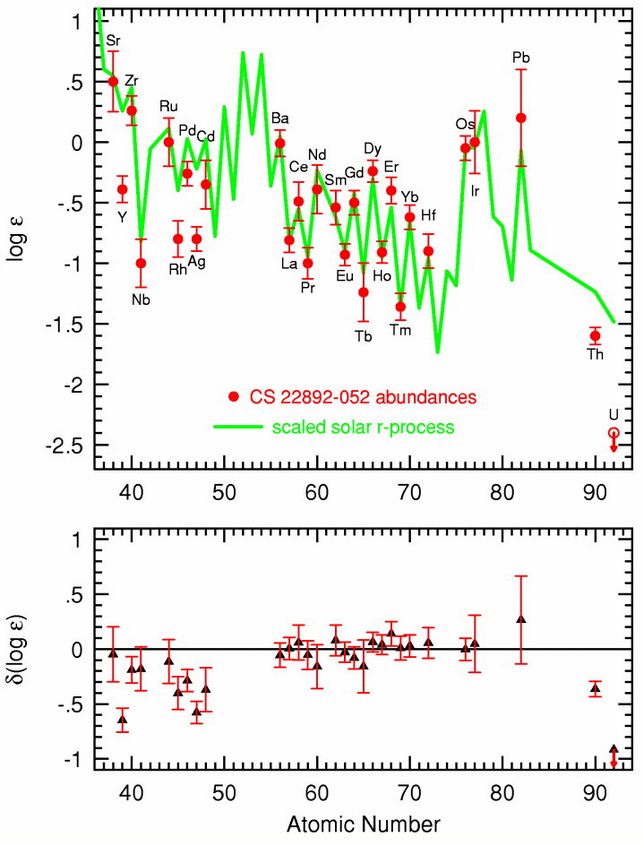
\includegraphics[width=\linewidth]{pdf/oldstar.png}
\caption{\label{fig:old} Data points represent measured heavy element
abundances from the metal-poor Galactic halo star CS 22892-052 while
the solid line represents the solar system r-abundance measurements,
scaled to fit the data points.  $\log \epsilon (x) \equiv log(N_x/N_H) +
12.0$ for a given element $x$.  Residuals are shown in the bottom
plot.  From~\cite{truranetal2002}.}
\end{figure}

Let us examine the requirements of the r-process.  Neutron captures
must proceed at a rate quicker than \bminus\ decay rates but also must
only happen for a limited amount of time, otherwise it is easy to
image scenarios where nuclides are ``over-processed'' and become very
heavy on average with a large abundance near Pb end of the valley of
stability and fission products of heavier nuclei, which is not seen in
the abundances.  Thus, the r-process must proceed quickly enough to
have the neutron capture rate greater than the \bminus\ decay rate yet
short enough that it doesn't create pile ups of heavy
elements. \cite{iliadis2008} quotes $\approx$seconds.
 Assume that, on average, each seed nucleus captures
100 neutrons over the course of the r-process and that the r-process
is in operation for 1 second we can calculate what
combinations of neutron capture cross section, neutron velocity
(dependent on temperature), and
neutron density can produce this.  If $m$ is the number of
interactions per nucleus we can write
\begin{equation}
\frac{m}{t} = N_n \langle \sigma v \rangle
\end{equation}
or
\begin{equation}
100 ~\textrm{s}^{-1} = N_n \langle \sigma v \rangle.
\end{equation}

The Galactic mass of r-processed material in the galaxy is also an
important observational constraint on r-process
sites.  \cite{meyer1994} gives the mass fraction of r-processed
material as $2\times 10^{-7}$.  Following their calculation (where they
quote a value of $1.5\times10^{11}$\Msol\ for the mass of the galaxy)
that means there is $\sim 10^4$\Msol\ of material formed from the
r-process in the Milky Way.  The supernova rate in our galaxy is
somewhere in between one a decade and one a century
(\citealt{van1991}) and our galaxy's age is on the order of the age of
the universe ($\sim 10^{10}$ years).  Bringing these all together it
is calculates that if supernovae are the primary r-process site then
each supernova must produce $10^{-5}-10^{-4}$\Msol\ of r-processed
nuclides. 

Supernovae need to produce very neutron rich (with electron fraction
$Y_e\lesssim 0.2$) to make the nuclei of the actinide series
(\citealt{meyer1994}).  In order for such neutron rich material to be
available from the core, a supernova would need to  throw out $\sim 0.1$\Msol\ of
r-processed material, overproducing observed r-process abundances by a
factor of $10^3$ based on our calculation above.  Proposals that only
certain supernovae, such as those with high magnetic fields and
rotation rates (\citealt{symbalistyetal1985}) can eject the neutron-rich matter have
been made but it is unknown whether populations of such objects exist
in the right manner to produce the observed abundances. 

The proto-neutron star that is formed as the result of a core collapse
supernova is very hot and can have a neutrino-driven wind
(\citealt{meyer1994}). However, this scenario has a difficult time
producing the correct abundance distribution for expected proto-neutron
star masses of 1.4\Msol\ and radii of 10 km (\citealt{thompson2001}).
Specifically they calculate that in order to produce the third peak
($A\sim 195$) abundances that the r-process must occur at early times,
with a modest entropy of $\sim 150~k_B$ per baryon, and with a short
dynamical timescale of $\sim1$ ms, conditions not met for a 1.4\Msol\
proto-neutron star.  They also find that the third r-process peak can
occur for proto-neutron stars with $M\gtrsim 2.0$ \Msol\ and radius
$\lesssim9$ km.  

Neutron star mergers are expect to eject some fraction of their mass
before coalescing; such neutron-rich material is a prime candidate for
an r-process site.  Binary neutron star systems are known to
exist (\citealt{thorsett1996}). \cite{rosswogetal1999} show that 
coalescing binary neutron stars
 create a thick disk of 0.1 to 0.3 \Msol\ made of
decompressed neutron star matter;
the material that becomes unbound from this disk is between
$4\times10^{-3}$ and $4\times10^{-2}$\Msol, depending on the initial
spins of the neutron stars for a realistic equation of state.  However they also show that for a test
 case of a soft polytrope ($\Gamma=2.0$) that there is no mass thrown
 from the merger, suggesting a strong dependence of the mass loss on
 the (as yet) unknown equation of state.  The ejected material has
 very large densities ($10^{12}-10^{14}$ g cm$^{-3}$) and low electron
 fraction ($Y_e<0.05$).  Such high density, neutron-rich material is a
 strong candidate for an r-process cite.  We can calculate whether
 such an amount of material cast off a neutron star merger can, by
 itself, account for the observed r-process abundance.  Using the
 neutron star merger rate given in \cite{price2006} (which is $4$ to
 $220\times10^{-6}$ per year and galaxy) and assuming a constant
 neutron star merger rate over the last $\sim 10^{10}$ year history of
 the Galaxy, that $\sim2\times10^2$ to $\sim9\times10^4$ \Msol\ of
 r-processed material could have been created in our Galaxy due to
 neutron star merges, with the large uncertainty in this calculation
 originating from uncertainties in the merger rate and amount
 of material released from a merger. The high end of this range is consistent with the previously
 calculated value for the amount of r-process material in the Galaxy,
 $\sim 10^4$\Msol.  Thus, neutron star mergers can possibly account for all
 r-processed nuclides in the Galaxy; the conclusion of this matter,
 though, is highly dependent on what the neutron star merger rate
 actually is.  Gravitational wave detectors such as LIGO and Virgo are
 expected to measure this rate.  Additionally, such an event may have
 recently been observed close by.  \cite{berger2013} suggest that the short-hard
 GRB 130603B may have been an r-process kilonova from a binary neutron
 star or neutron star-black hole merger.

%  LocalWords:  bminus nuc iliadis2008 saha lambdaz th meyer1994 Msol
%  LocalWords:  firsttermination secondtermination lesssim-2.5
%  LocalWords:  truranetal2002 symbalistyetal1985 thompson2001
%  LocalWords:  thorsett1996 rosswogetal1999
